\section{Evaluation} \label{sec:evaluation}
\textcolor{red}{Hier fehlt die Einführung, Britta}

\subsection{Tasks} \label{sec:tasks}
The supermarket (compare section~\ref{sec:supermarket}) is confronted with four tasks. In every task, an object has to be selected and placed on a target area. If the correct object is placed, the target area will change the color to signal that the tasks is successful done. In the script \textit{TargetTest.cs}, which is added as a component to the target object, is recognized when the target object hits the target area. At this moment the texture of target area is changed and the measurement (compare section~\ref{sec:measurement}) is stopped. \\
In the first three tasks the user has to select different objects. Therefore the user can decide which method he/she uses to grab the object. The selected method should differ depending on the tasks. In these tasks objects far away as well as in the CR should be picked. \\
The tasks will be shown next to the controller similar to the selfteaching (compare section~\ref{sec:selfteaching}), which the user is already aware of. The placement of the tasks is shown in the following figure. 

\begin{figure}[H] 
	\center 
	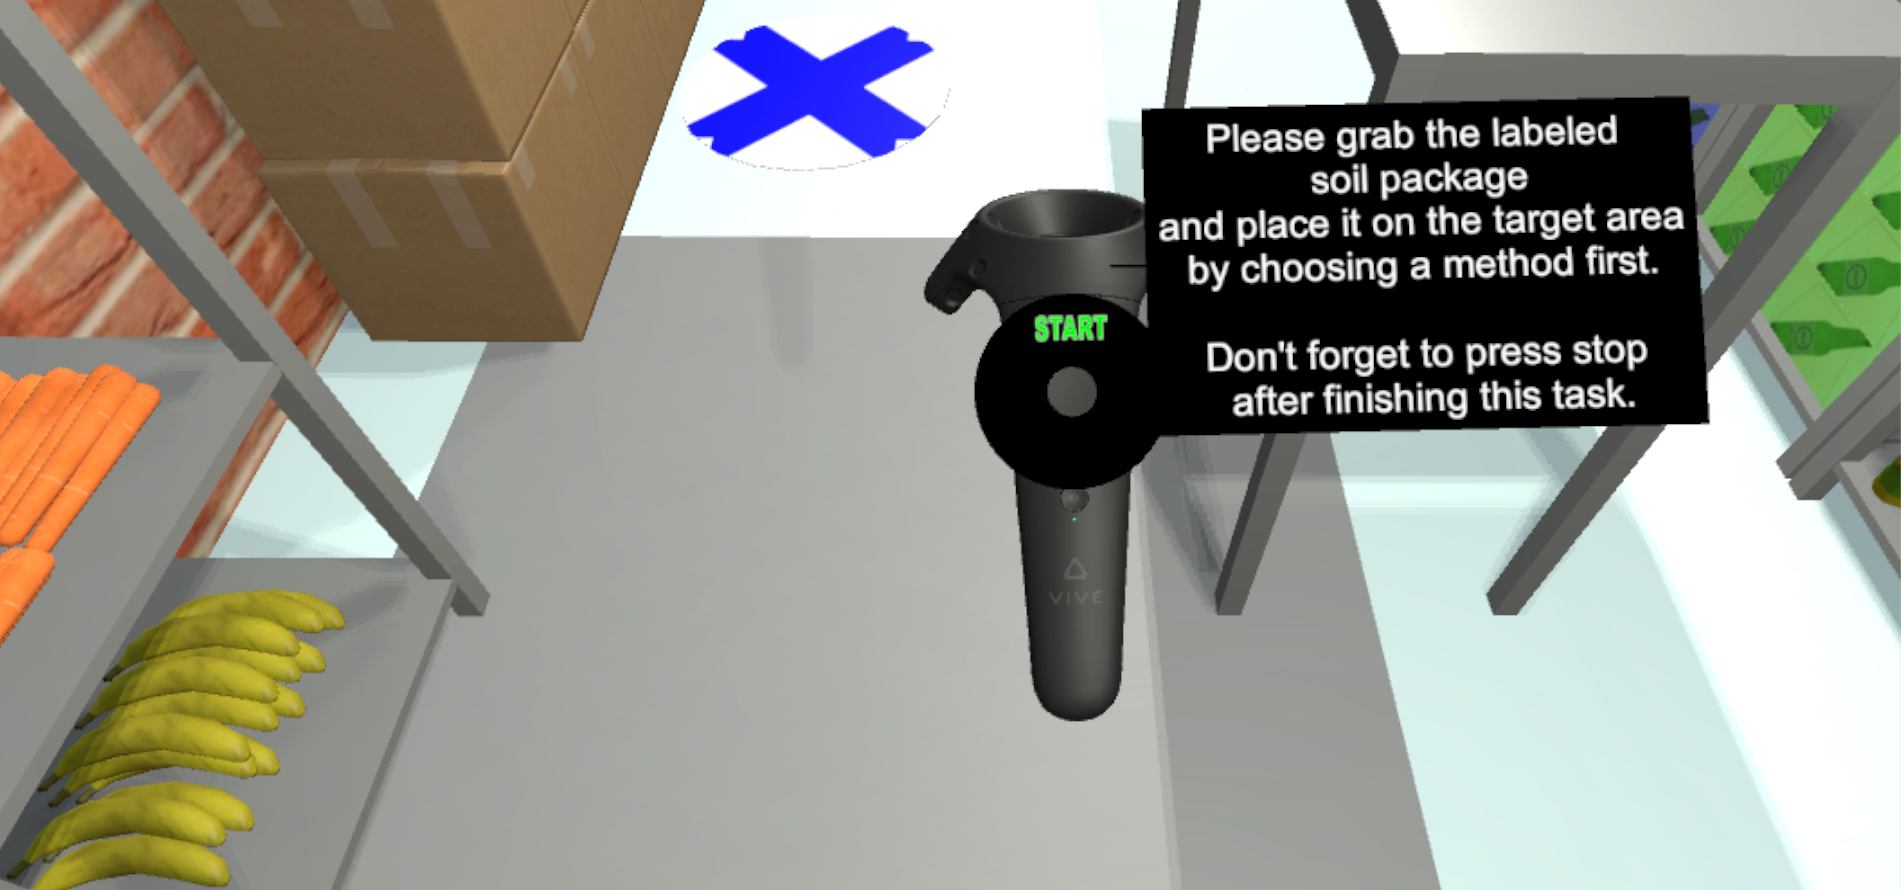
\includegraphics[width=12cm]{Images/TaskContreoller.PNG}
	\caption[Task shown next to the Controller.]{Task shown net to the Controller.}
	\label{fig:taskC}
\end{figure} 

The text for the tasks are saved in a CSV-file, similar to the selfteaching, see section \ref{sec:selfteaching}. The implementation is also comparable to the selfteaching and implemented in the script \textit{showTasks.cs}.

\begin{figure}[H] 
	\center 
	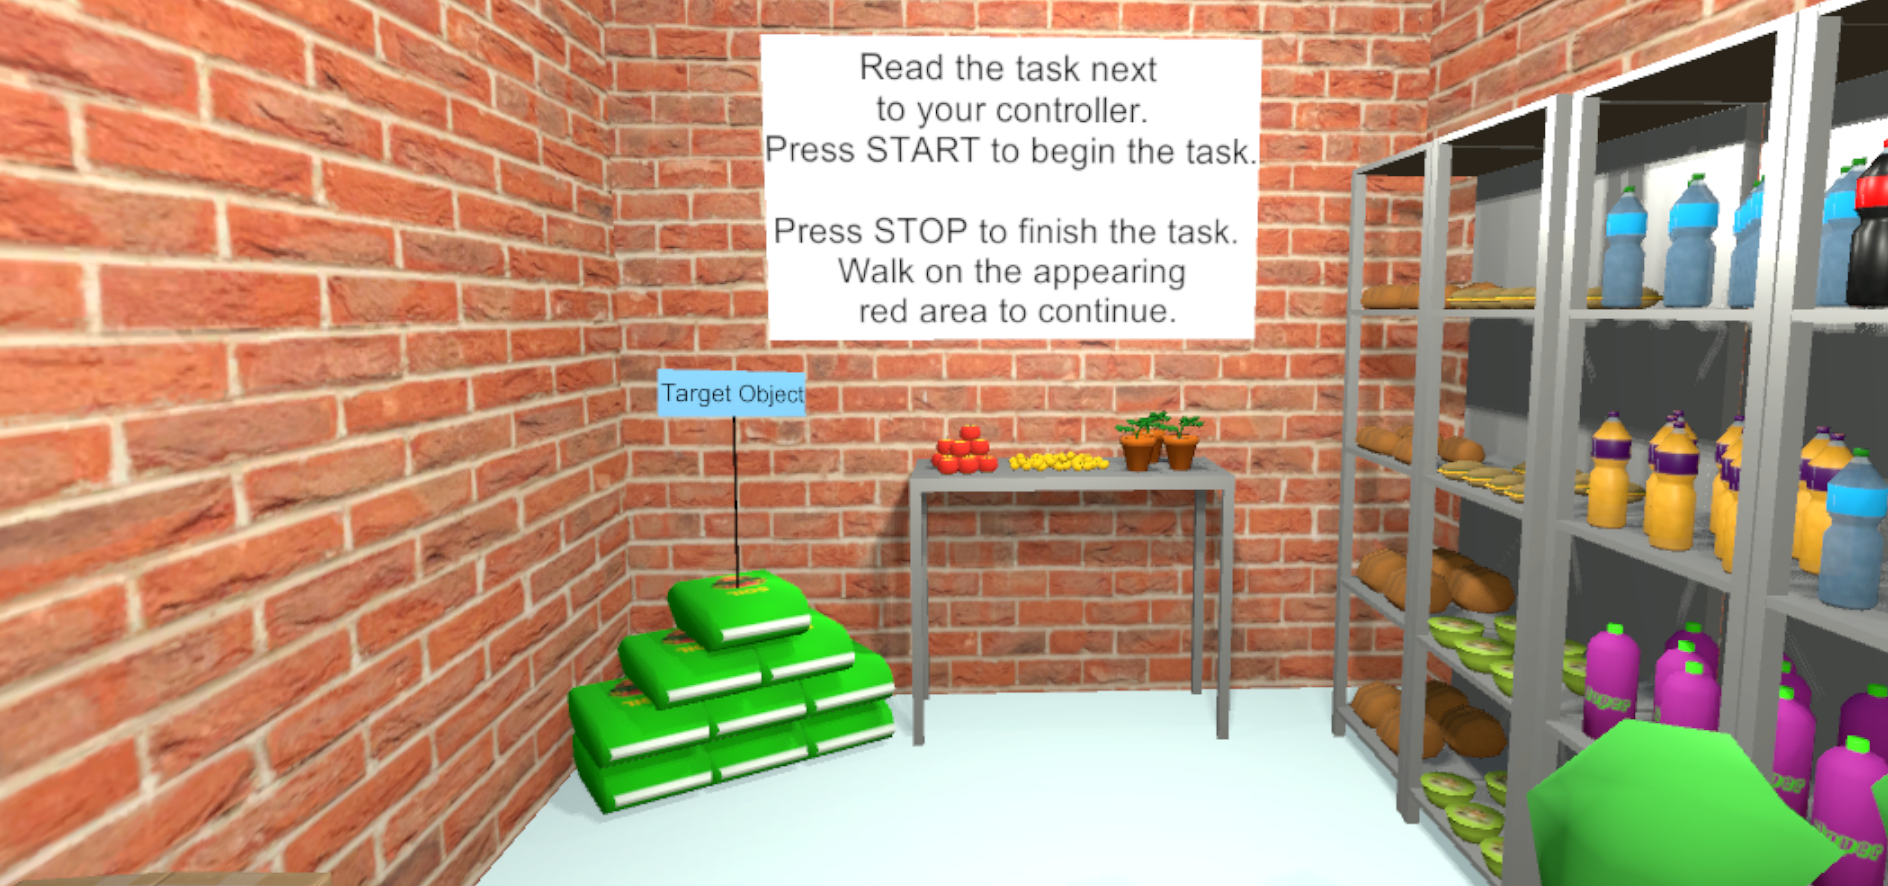
\includegraphics[width=12cm]{Images/TaskWall_1.PNG}
	\caption[Additional Information on the Wall.]{Additional Information on the Wall.}
	\label{fig:taskW1}
\end{figure}

To give the user some more instructions a information board within the supermarket is established, see figure \ref{fig:taskW1}. For the first three tasks there are only shown some basic information.\\
The last tasks will be repeated with every available method. That means, that the user has to pick up the same object five times. This object is placed, so that the user could use CR as well as FR methods (compare section~\ref{sec:Interactions}. The methods are implemented in a fix order which can be seen in table \ref{tab: OrderMethods}. The methods will already be activated as soon as the user presses start. \\

\begin{table}[h]
\centering
 \begin{tabular}{|c|c|}
  Number of subtask & Method  \\ \hline
  1 & Close Range: Touch Grab  \\
  2 & Close Range: Wand Grab  \\
  3 & Far Range: Extendable Ray  \\
  4 & Close Range: Proximity Grab  \\
  5 & Far Range: Raycast \\
   \end{tabular}
  \caption[Order of methods in the last tasks.]{Order of methods in the last tasks.}
	\label{tab: OrderMethods}
 \end{table}

To help the user to figure out what method is activated the name of the method will be shown on the information board as soon as  he is in the new scene (compare figure~\ref{fig:taskW2}). 

\begin{figure}[H] 
	\center 
	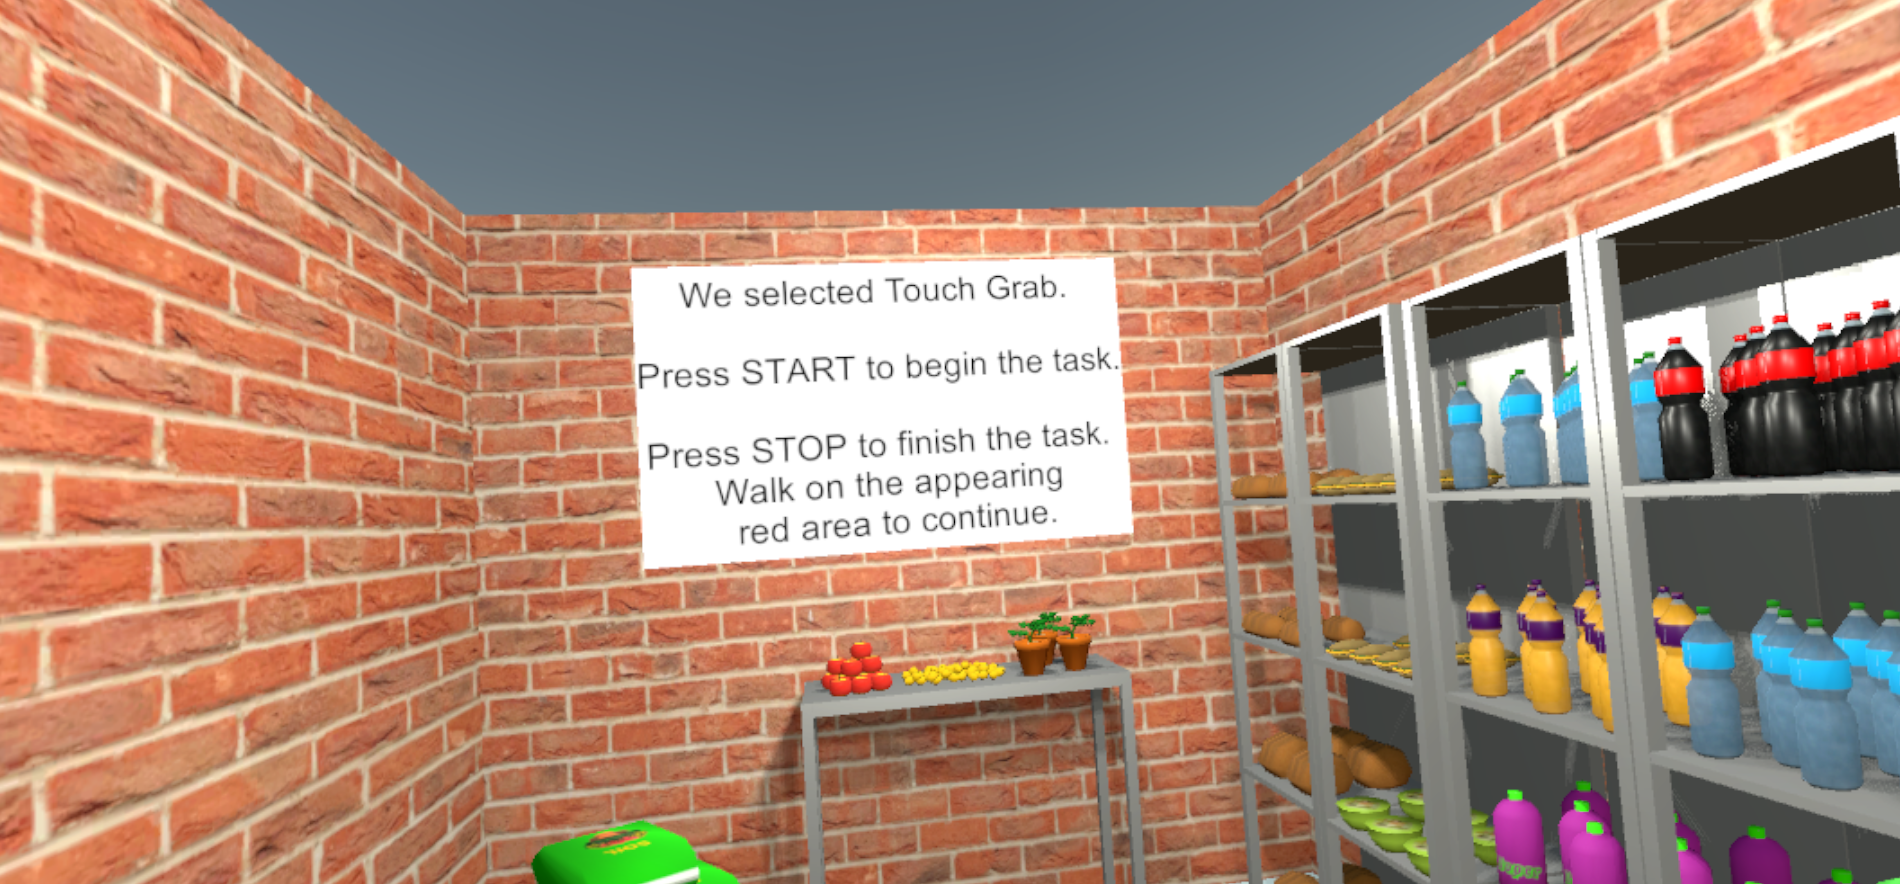
\includegraphics[width=12cm]{Images/TaskWall_2.PNG}
	\caption[\textit{Touch Grab} is activated.]{\textit{Touch Grab} is activated.}
	\label{fig:taskW2}
\end{figure}

For the last tasks a usability questionnaire needs to be answered by the user, after he finishes the task. 


\subsection{Measurement} \label{sec:measurement}

\subsubsection{Time and Precision Measurement}
\todo[inline, color=yellow]{Vera}
As mentioned in section \ref{sec:tasks} the users has to fulfil several tasks which are designed to evaluate various aspects. Thus three different sets of measurements will be saved automatically in a task. All results are stored in a comma separated value text file that is named after their subtask and stored directly into the unity project folder. These files can be imported in all common statistic applications like \textit{MS Office Excel}, for example. Hence, the provided template is a \textit{Excel} file with the required basic statistic computations and visualisation of the results. Here, the output files could be easily integrated in the designated table fields. Following this, the template computes all useful mean values and standard deviations of the measurements. In other cases, it calculates the percentagewise proportion like the commonness of a method use. Each calculation is displayed in a corresponding diagram. Further, the ones that visualise the mean values includes an error bar that depends on the standard deviation. If necessary, other static computation like a significance test needs to be extended because the calculation highly depends on the study conditions and are not predictable.

The first measuring set is made for the learning procedure and evaluates the affordable learning time of a grabbing method. Therefore their usage time is recorded during the complete learning process and saved in milliseconds when a user presses the stop button. 

Afterwards the first task with its three subtasks is started. Here the user's method preference of a close or far range task will be evaluated. Hence the application measures the usage time of every selected method and saves the id of the current method when the target object is placed successfully on the target area. The listing of this measurement shows significantly which methods were preferred and if a user had comprehend their scope.  

Finally the precision as well as the grabbing and positioning time is measured in the second task for every provided method. Therefore the grabbing time is started when a user presses the start button and stopped when the target object is grabbed. At this point the positioning time is started immediately and stopped when the object is placed on the target area. These time measuring  shows the workload and where the users have problems with the method. Additional the selecting and positioning error rate is recorded during the whole process. Thus this recorded data gives conclusions about the precision. The success of this task is recorded and the use of the snapping mode, too. Hence all relevant informations are provided to get all important conclusions about the applicability of each method. 

\subsection{Questionnaires} \label{sec:questionnaires}

\textcolor{red}{Hier wäre es generell schöner einen flüssigere Überleitungen zuschreiben. Meisten benutzt du drei bis viermal hintereinander "The" als Textanfang oder immer gleiche Satzmuster wie z.b. THe evaluation Formula... is intergrated oder "This is done ... !. }
To not only use measured values to evaluate the interaction methods but also use the participants input, the participants have to fill out two kinds of questionnaires. The first one is the \textit{SUS: a 'quick and dirty' usability scale} usability questionnaire \citep{6sus}. This questionnaire consists of ten questions. It is given to the user after each task, so each user fills out the questionnaires five times, once for each interaction method. \textcolor{red}{Hier könnte man zum besseren Verständnis etwas genauer sein. Vorallem, dass der Fragebogen im zweiten Task direkt nach der Benutzung der jeweiligen Methode ausgefüllt wird.}This is done to determine the usability of each method. The investigator has to fill in two extra questions which are a testID (one number assigned to every participant) and which method was used \textcolor{red}{Wann genau muss er das machen? oder andere Reihenfolge in der Beschreibung der Fragebögen}.This is done to be able to draw an conclusion based on the used method \textcolor{red}{Vorschlag: Hence, it is possible to draw a conclusion based on the used method.}  \\ 

The second questionnaire is a simulator sickness questionnaire by Kennedy et al. \citep{ssq} which evaluates the general discomfort caused by the virtual reality application. The investigator has to fill in the testID corresponding to the testID used for the usability questionnaire \textcolor{red}{Hier könnte man auch schreiben: This questionnaire has to be handed to the participant after all tasks are completed and the corresponding testID is entered by the investigator. Oder so ähnlich. Auf jeden Fall nicht dreimal "The" am Satzanfang}. \\

The \textcolor{red}{Durch All ersetzen?} questionnaires can either be used in a printed paper form or the provided \textit{Google Forms} can be utilized on a mobile device. When done in \textit{Google Forms}, the result can be imported into \textit{MS Office Excel}. Moreover, evaluation templates are provided as \textit{Excel} files with basic statistic calculations and visualisations. The evaluation formula \textcolor{red}{Besser: calculations or computations} of the simulator sickness questionnaire are integrated and could be easily applied to larger study groups. The result consists of four values: nausea, optic, disorientation and the total score. The total score has a range from 0 to 160.7, but a theoretical result of over 100 would be so dangerous that an ambulance should be called. \\
The evaluation formula for the usability questionnaire is also integrated. The resulting value has a range from $0$ to $100$ whereas a value of $100$ is considered for a perfect system. Above 70 are systems with good usability and a score under 50 indicates huge deficit in usability. \textcolor{red}{Vorschlag: In general, systems with a value of more than 70 seems to have a good usability and systems wit a score under 50 have a huge deficit.} \textcolor{red}{Wieder Viermal The am Anfang :-(}




\newpage